\documentclass{article}
\usepackage[utf8]{inputenc}
\usepackage{enumitem}
\usepackage{amsmath,amsthm,amssymb}
\usepackage[english]{babel}
\usepackage[a4paper, portrait, margin=1.2in]{geometry}
% \usepackage{ntheorem}
% \usepackage{theoremref}
\usepackage{xifthen}
\usepackage{relsize}
\usepackage[svgnames]{xcolor} % You can find CSS colours here https://www.w3schools.com/cssref/css_colors.asp

\usepackage{tkz-euclide}
\usepackage{tikz}
% \usepackage{showframe} % Useful for debugging

\usepackage{titlesec}
% \usepackage{caption}
\definecolor{MainColor}{hsb}{0, 0.8, 0.65}
\definecolor{SubColor}{hsb}{0.01, 0.90, 0.45}
\definecolor{SubSubColor}{hsb}{0.01, 0.90, 0.2}
% \usepackage[labelfont={color=SubColor,bf}]{caption}
\usepackage[labelfont={color=SubColor,bf}]{caption}

% switch implementation from https://tex.stackexchange.com/questions/64131/implementing-switch-cases
\newcommand{\ifequals}[3]{\ifthenelse{\equal{#1}{#2}}{#3}{}}
\newcommand{\case}[2]{#1 #2} % Dummy, so \renewcommand has something to overwrite...
\newenvironment{switch}[1]{\renewcommand{\case}{\ifequals{#1}}}{}

% \titleformat{\section}[block]
% {\bfseries\color{MainColor}}
% {\thesection.}{0.5em}{}[]

\newcommand{\hint}{\\\textcolor{SubColor}{{H}{\relsize{-1}INT:}}\ }

\renewcommand*{\thesection}{\textcolor{MainColor}{\arabic{section}}}
% \renewcommand*{\mySection}[1]{\section{\textcolor{MainColor}{#1}}}
\newcommand{\solution}{\subsubsection*{\textcolor{MainColor}{Solution}}}
% \renewcommand{\figurename}{\textcolor{SubColor}{Fig.}}
% \renewcommand{\thefigure}{\textcolor{ocre}{\bfseries\itshape\thechapter.\arabic{figure}}}
% \renewcommand{\figurename}{\textcolor{ocre}{\bfseries\itshape Fig.}}

% \captionsetup{
%   format=plain,
%   justification=raggedright,
%   singlelinecheck=false,
%   font=small,
%   font={bf,sf}, % This covers labelfont and textfont
%   labelsep=pipe,
%   figurename=Figure
% }

\newcounter{theoremcounter}

\newtheoremstyle{maintheorem}% name of the style to be used
	{\topsep}% measure of space to leave above the theorem. E.g.: 3pt
	{\topsep}% measure of space to leave below the theorem. E.g.: 3pt
	{\itshape}% name of font to use in the body of the theorem
	{0pt}% measure of space to indent
	{\color{SubColor}\bfseries}% name of head font
	{.}% punctuation between head and body
	{ }% space after theorem head; " " = normal interword space
	{\thmname{#1}\thmnumber{ #2}\textnormal{\thmnote{ (#3)}}}

\theoremstyle{maintheorem}
\newtheorem{theorem}[theoremcounter]{\textcolor{SubColor}{Theorem}}
\newtheorem{corollary}{\textcolor{SubColor}{Corollary}}


\newcommand{\thmref}[1]{\textcolor{SubSubColor}{\textbf{Theorem \ref{#1}}}}
\newcommand{\corref}[1]{\textcolor{SubSubColor}{\textbf{Corollary \ref{#1}}}}
\renewcommand{\eqref}[1]{\textcolor{SubSubColor}{\textbf{Equation \ref{#1}}}}

% \theoremstyle{mainsolution}
% \newtheorem*{solution}{Solution}



\newcommand{\size}[2]{
	\begin{switch}{#1}
		\case{1}{#2}
		\case{2}{\bigl#2}
		\case{3}{\Bigl#2}
		\case{4}{\biggl#2}
		\case{5}{\Biggl#2}
	\end{switch}
}

\setlength{\parskip}{0.8em}


\title{Babak's Problem}
\author{Rasmus Söderhielm}
\date{December 2021}

\begin{document}
\maketitle

% \begin{figure}
%     \begin{tikzpicture}
%         % Every aspect of the figure can be altered through these definitions
%         \def\radius{3} \def\X{0.35} \def\labelSpacing{1.1}
%         \def\A{110} \def\B{315} \def\C{70} \def\D{215}

%         % Restricts the canvas
%         \tkzInit[xmin=-3.25,xmax=3.25,ymin=-3.25,ymax=3.25]\tkzClip

%         \tkzDefPoints{0/0/O, \radius/0/R} % defines the first two points

%         % The remainder of the points are defined through rotation
%         \tkzDefPointBy[rotation=center O angle \A](R)\tkzGetPoint{A}
%         \tkzDefPointBy[rotation=center O angle \B](R)\tkzGetPoint{B}
%         \tkzDefPointBy[rotation=center O angle \C](R)\tkzGetPoint{C}
%         \tkzDefPointBy[rotation=center O angle \D](R)\tkzGetPoint{D}

%         % Get the point M as the intersection between the lines AB and CD
%         \tkzInterLL(A,B)(C,D)   \tkzGetPoint{M}

%         % Calculate the length AD, and define the point X
%         % as X = 0 at A and X = 1 at D
%         \tkzCalcLength[cm](A,D) \tkzGetLength{dAD}
%         \pgfmathparse{\X*\dAD}
%         % Intersect between circle with center A and radius \X * AD
%         \tkzInterLC[R](A,D)(A,\pgfmathresult cm) \tkzGetPoints{X'}{X}

%         % Finds the intersection for PQ in a similar fashion, same with Y
%         \tkzInterLC(X,M)(O,R)                    \tkzGetPoints{P}{Q}
%         \tkzInterLL(X,M)(C,B)                    \tkzGetPoint{Y}

%         \tkzDrawPoints[fill=black,size=7pt](A,B,C,D,X,Y,P,Q,M)

%         \tkzMarkAngle[size=1.5cm, arc=lll](C,D,A)
%         \tkzMarkAngle[size=1cm, arc=lll](C,B,A)

%         \tkzMarkAngle[size=0.5cm, arc=ll](X,M,D)
%         \tkzMarkAngle[size=0.5cm, arc=ll](Y,M,C)

%         \tkzMarkAngle[size=0.4cm, arc=l](A,M,X)
%         \tkzMarkAngle[size=0.4cm, arc=l](B,M,Y)

%         \tkzDrawSegments(A,B B,C C,D D,A P,Q)
%         \tkzDrawCircle(O,R)

%         % This just defines the labels radially, looks slightly better
%         \node at ($(O)+\labelSpacing*(A)$)  {$A$};
%         \node at ($(O)+\labelSpacing*(B)$)  {$B$};
%         \node at ($(O)+\labelSpacing*(C)$)  {$C$};
%         \node at ($(O)+\labelSpacing*(D)$)  {$D$};
%         \node at ($(O)+\labelSpacing*(P)$)  {$P$};
%         \node at ($(O)+\labelSpacing*(Q)$)  {$Q$};

%         \tkzLabelPoints[above=0.2cm](M)
%         \tkzLabelPoints[above left](X)
%         \tkzLabelPoints[above right](Y)
%     \end{tikzpicture}
%     \caption{Picture From Forum}
% \end{figure}
% \begin{figure}
%     \begin{tikzpicture}
%         \def\ang{30}

%         \tkzInit[xmin=-1,xmax=6,ymin=-1,ymax=5]
%         \tkzClip

%         \tkzDefPoint(0,0){O}

%         % Draw axis
%         % \tkzAxeXY[step=2]
%         \tkzDrawX\tkzLabelX[orig,step=2]
%         \tkzDrawY\tkzLabelY[orig,step=2]

%         % Define function intersection point.
%         \tkzDefPoint(4,2){P_0}
%         \tkzDrawPoints(P_0)\tkzLabelPoints(P_0)

%         \tkzDefPoint(10,0){V_0}
%         \tkzDefPointWith[colinear=at P_0](O,V_0) \tkzGetPoint{M_1}
%         \tkzDefPointBy[rotation=center P_0 angle \ang](M_1) \tkzGetPoint{L_1}
%         \tkzDefPointWith[colinear=at P_0](V_0,O) \tkzGetPoint{M_2}
%         \tkzDefPointBy[rotation=center P_0 angle \ang](M_2) \tkzGetPoint{L_2}

%         \tkzDrawSegments(L_1,L_2)

%         % Get x-axis intersection
%         \tkzInterLL(O,V_0)(L_1,L_2) \tkzGetPoint{X}

%         % Mark angle
%         \tkzMarkAngle[size=0.8cm,mark=none](V_0,X,L_1)
%         \tkzLabelAngle[pos=1.2](V_0,X,L_1){$\ang^{\circ}$}

%         % \tkzDrawPoints(O,V_0,X,L_1)
%         % \tkzLabelPoints(O,V_0,X,L_1)

%     \end{tikzpicture}
%     \caption{My Own Picture}
% \end{figure}

\section{Description of the Problem}
We are given an isosceles triangle $ABC$ the angle $\angle BAC$ equal to $20^\circ$.
Let point $D$ be a point placed on the line segment $\overline{AB}$,
where the distance between the two points $A$ and $D$ is the same as the distance between $B$ and $C$.
Find the angle $\theta$ that is defined as the angle $\angle BDC$.

\begin{figure}[h]
    \centering
    % \begin{center}
    % \fbox{
    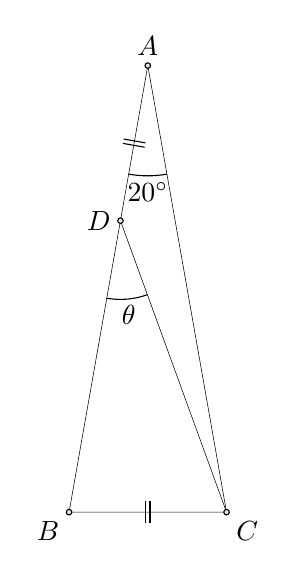
\begin{tikzpicture}[x=1cm,y=1cm]

        % \tkzInit[xmin=-0.5,xmax=3.5,ymin=-0.5,ymax=7.5]
        % \tkzClip

        \def\width{2}

        \tkzDefPoint(0,0){O}
        \tkzDefPoint(0,0){B}
        \tkzDefPoint(\width,0){C}

        \tkzDefTriangle[two angles=80 and 80](B,C) \tkzGetPoint{A}

        \tkzDefShiftPoint[A](-100:\width){D}


        \tkzDrawPolygon[](A,B,C)
        \tkzDrawSegments(D,C)

        \tkzDrawPoints(A,B,C,D)
        % \tkzLabelPoints(A,B,C,D)
        \tkzLabelPoints[above](A)
        \tkzLabelPoints[below left](B)
        \tkzLabelPoints[below right](C)
        \tkzLabelPoints[left](D)

        \tkzMarkAngle[size=1.4,mark=none](B,A,C)
        \tkzLabelAngle[pos=1.6](B,A,C){$20^{\circ}$}
        \tkzMarkAngle[size=1,mark=none](B,D,C)
        \tkzLabelAngle[pos=1.2](B,D,C){$\theta$}

        % \tkzFindAngle(C,B,A) \tkzGetAngle{angCBA}
        % \tkzFindAngle(A,C,B) \tkzGetAngle{angACB}
        % \tkzFindAngle(B,A,C) \tkzGetAngle{angBAC}
        % \tkzLabelAngle[pos=0.4](C,A,B){$\angBAC^{\circ}$}

        % \tkzMarkAngle[size=0.3, mark=0](C,B,A)
        % \tkzLabelAngle[pos=0.4](A,B,C){$\angCBA^{\circ}$}
        % \tkzMarkAngle[size=0.3, mark=0](A,C,B)
        % \tkzLabelAngle[pos=0.4](B,C,A){$\angACB^{\circ}$}

        \tkzMarkSegments[mark=||](A,D B,C)
    \end{tikzpicture}
    % }
    % \end{center}
    \caption{Babak's initial problem}
\end{figure}

\subsection{The Solution}

Let's begin by imagining making a copy of the triangle $ABC$, placing the transformed points $B'$ and $C'$ on the original points $A$ and $D$ respectively, giving us the triangle $ADE$.

The angle $\angle CAE$
We can conclude that the triangle $ACE$ is an isosceles.

\end{document}